\documentclass{article}
\usepackage[utf8]{inputenc}
\usepackage{graphicx}
\usepackage{amsmath}
\usepackage{listings}
\usepackage{caption}
\usepackage{subcaption}

\begin{document}

\begin{center}
    \huge
    \textbf{Modelling the Chaotic Behavior of Chua's Circuit}

    \vspace{0.3cm}    
    \large
    PHYS 4810 - Computational Physics
    
    \vspace{0.2cm}
    \large
    Aditri Bhat
\end{center}


\section{Introduction}
    Many real world systems have complex differential equations that have no closed analytical solution, and so we must turn to computational methods to understand and predict their behavior. One such example is Chua's Circuit, which is one of the simplest circuits to model chaotic behavior. This behavior arises due to a specific component within the circuit, known as a Chua's diode. This component has the special properties of being nonlinear and a locally active resistor, meaning that it has negative resistance\footnote{ http://www.chuacircuits.com/diagram.php}. A diagram of the circuit is shown below:
    
    \begin{figure}[h]
        \centering
        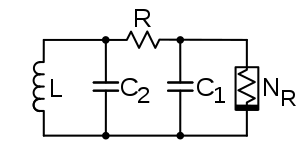
\includegraphics[scale = 0.6]{Images/chua_circuit.png}
        \caption{Chua's Diode is located to the right.}
        \label{fig:my_label}
    \end{figure}
    
    The main variables of interest are related to the two capacitors and the inductor. Solving out for these gives a set of three highly coupled equations:
    
    $$\frac{dx}{dt} = \alpha[y - x - f(x)]$$
    $$RC_2\frac{dy}{dt} = x - y + Rz$$
    $$\frac{dz}{dt} = -\beta y$$
    
    In these equations, x and y represent the voltages in capacitors one and two respectively, and z represents the current of the inductor. The parameters $\alpha$, $\beta$ and $f(x)$ are dependent on the physical parameters of the Chua's diode. This set of equations is known as the dimensionless form, while the explicit form is shown below:
    
    $$\frac{dV_1}{dt} = \left(\frac{1}{R*C_1}\right)(V_2 - V_1 - R*g(V_1))$$
    $$\frac{dV_2}{dt} = \left(\frac{1}{R*C_2}\right)(V_1 - V_2 + RI_L)$$
    $$\frac{dI_L}{dt} = -\frac{V_2}{L}$$
    
    \[g(V_1) = 
        \begin{cases} 
          m_0V_1 + (m0 - m1)E_1 &\quad V_1\leq -E_1 \\
          m_1V_1 &\quad -E_1 < V_a < E_1\\
          m_0V_1 + (m_1 - m_0)E_1 &\quad E_1\leq V_1 
       \end{cases}
    \]
    \medskip
    
    Implementing this form of the equations is more difficult, though in regards to physical testing, it is more useful. Overall, the goal of simulating this system is to show that it truly is a chaotic system, namely that small changes to the initial conditions induce a large change in the solution. As such, in the algorithm, we hope to utilize an accurate method of solving these coupled ODES and provide visualizations for this system.

\section{Algorithms and Code}

    One of the main things to consider first is which ODE solving method to utilize. There are many available methods, such as Euler's method, Runge-Kutta methods, and other more unique methods, such as implementing a convolutional neural network. Due to the complexity of the system, we will be utilizing \verb|odeint()| from \verb|scipy.integrate|. \verb|odeint()| utilizes LSODA as the main solution method, which dynamically selects between nonstiff and stiff methods\footnote{https://github.com/scipy/scipy/blob/v0.19.0/scipy/integrate/odepack/readme}. In the nonstiff method, it utilizes Adams methods, which use polynomial interpolation. For the stiff case, it utilizes backwards differentiation formulas. Overall, the combination of the two leads to an efficient algorithm for solving a system of ODEs. 
    
    One of the requirements of \verb|odeint()| is a function that provides the derivatives of all variables for a given state and time. The code is shown below:
    \newpage
    
    \begin{lstlisting}[language=Python]
        def deriv(r, t, alpha, beta, M0, M1):
        
            x, y, z = r.copy()
            drdt = np.zeros(3)
            
            h = M1*x + (abs(x+1) - abs(x-1))*(M0 - M1)/2
            drdt[0] = alpha * (y-x-h)
            drdt[1] = (x-y+z)
            drdt[2] = -beta * y
        
        return drdt
    \end{lstlisting}
    
    If we consider an actual circuit (shown below) for which we would like to predict its behavior, we may also implement the realistic form of the equations with the following code:
    
    \begin{figure}[h!]
        \centering
        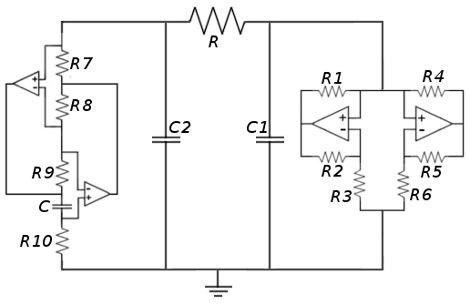
\includegraphics[scale = 0.5]{Images/simulated_circuit.png}
        \caption{The circuit to be simulated.}
        \label{fig:my_label}
    \end{figure}
    
    \begin{lstlisting}[language = Python]
        def deriv_real(r, t, batt_V = 9):
    
        x, y, z = r.copy()
        drdt = r.copy()
        
        # Defining the constants
        
        C1  = 10e-9        # 10nF
        C2  = 100e-9       # 100nF
        R = 1800           # 1.8k Ohms
        G = 1/R
        
        # Constants relating to the Chua Diode
        
        R1 = 220
        R2 = 220
        R3 = 2200
        R4 = 22000
        R5 = 22000
        R6 = 3300
        
        EV = batt_V             # 9V Batteries
        E1 = R3/(R2+R3)*EV
        E2 = R6/(R5+R6)*EV
        
        m12 = -1/R6
        m02 = 1/R4
        m01 = 1/R1
        m11 = -1/R3
        
        m1 = m12 + m11
        
        if E1 > E2:
            m0 = m11 + m02
        else:
            m0 = m12 + m01
        
        mm1 = m01 + m02
        Emax = max(E1, E2)
        Emin = min(E1, E2)
        
        if abs(x) < Emin:
            const = x*m1
        elif abs(x) < Emax:
            const = x * m0
            if x > 0:
                const += Emin * (m1-m0)
            else:
                const += Emin * (m0-m1)
        
        elif abs(x) >= Emax:
            const = x * mm1
            if x > 0:
                const += Emax*(m0-mm1) + Emin*(m1-m0)
            else:
                const += Emax*(mm1-m0) + Emin*(m0-m1)
                
        # Constants relating to the Gyrator
        
        R7  = 100              #100 Ohms
        R8  = 1000             #1k Ohms
        R9  = 1000             #1k Ohms
        R10 = 1800
        C   = 100e-9           #100nF
        L = R7*R9*C*R10/R8     #18mH 
        
        # Returning the derivative
        
        drdt[0] = (G*(y-x) - const)/C1
        drdt[1] = (G*(x-y)+z)/C2
        drdt[2] = -y/L
        
        return drdt
    \end{lstlisting}
    
    One of the heavy drawbacks to utilizing the realistic form of the Chua's circuit equations is the number of constants required. In comparison to the few that the dimensionless version has, the realistic form has multiple constants that depend on the physical parameters of the circuit. For a more complex circuit that still follows the same general dimensionless form, the realistic version would have even more constants, something that could be an issue in regards to human error. 
    
    
    The dimensionless implementation allows for the input of the constants, thus being able to shift the system and see what changes. With this, we can use \verb|odeint()| in the code below:
    \begin{lstlisting}
        r0 = [0.7, 0, 0]
        t = np.linspace(0, 30, 10000)
        const = (15.6, 28, -1.143, -0.714)
        r = odeint(deriv, r0, t, args = const)
        
        x = r[:, 0].T
        y = r[:, 1].T
        z = r[:, 2].T
    \end{lstlisting}
    
    We can use a similar method with the realistic version to compare. 
    
    \medskip
    \newpage
\section{Results}

    Now, we can graph the results to see how the variables evolve with time. 
    
    \begin{figure}[h!]
        \centering
        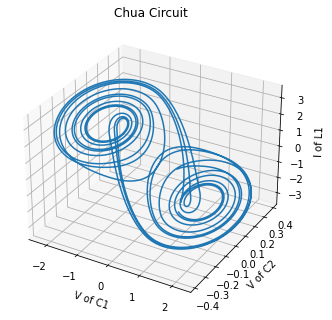
\includegraphics[scale=0.6]{Images/initial.png}
        \caption{A 3D plot of the voltages and current.}
        \label{fig:my_label}
    \end{figure}

    Another consideration is how the system appears in regards to just two variables - the graph below shows the relation between the two voltages. 
    
    \begin{figure}[h!]
        \centering
        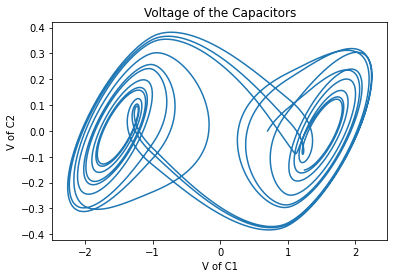
\includegraphics[scale = 0.6]{Images/projectionxy.png}
        \caption{Comparison of the two voltages.}
        \label{fig:my_label}
    \end{figure}
    
    Within both of these figure, we can notice two major areas of high density. It appears to stay within one of the two regions, before rapidly shifting to the other, at a seemingly random interval. One thing to consider is how initial conditions affect the results - would a small change in the x cause a large perturbation within the solution? By varying the initial values slightly, we can notice a significant shift. 
    
    \begin{figure}[h!]
        \centering
        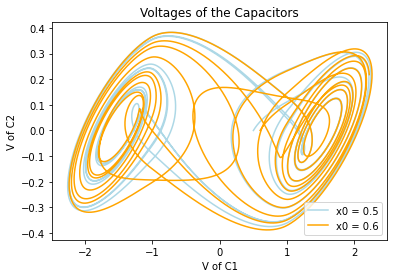
\includegraphics[scale=0.6]{Images/combined.png}
        \caption{Both $x=0.5$ and $x=0.6$ combined.}
        \label{fig:my_label}
    \end{figure}
    
    \begin{figure}[h!]
        \centering
        \begin{subfigure}[b]{0.4\textwidth}
            \centering
            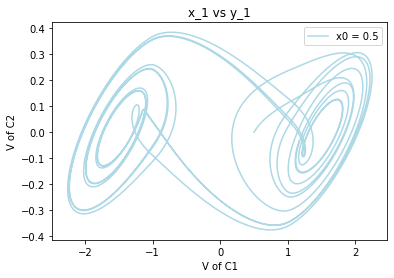
\includegraphics[width=1.4\textwidth]{Images/separate1.png}
            \caption{The $x = 0.5$ case.}
            \label{fig:my_label}
        \end{subfigure}
        \hfill
        \begin{subfigure}[b]{0.4\textwidth}
            \centering
            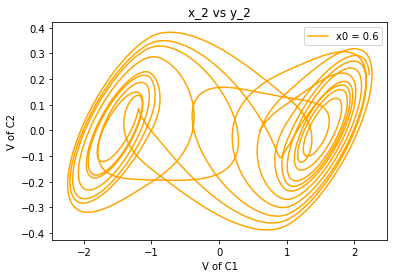
\includegraphics[width=1.4\textwidth]{Images/separate2.png}
            \caption{The $x = 0.6$ case.}
            \label{fig:my_label}
        \end{subfigure}
    \end{figure}
    
    Although both the graphs look similar, there is a significant change in that the $x=0.6$ case appears to shift between the two major states much more often. As this was due to purely a small change in the initial conditions, we can conclude that this is a chaotic system. We can confirm this with the results for the realistic form of the equations, which show a very similar pattern. 
    
    \begin{figure}[h!]
        \centering
        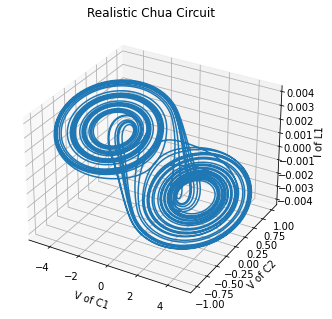
\includegraphics[scale = 0.6]{Images/realistic.png}
        \caption{The realistic implementation.}
        \label{fig:my_label}
    \end{figure}

    \newpage


\section{Drawbacks and Conclusion}

    One of the main things to consider is whether the simulated behavior lines up with the actual expected behavior. When measured with an oscilloscope, the results match up exactly with the predictions of the model\footnote{http://www.chuacircuits.com/pix.php}. 
    \begin{figure}[h!]
        \centering
        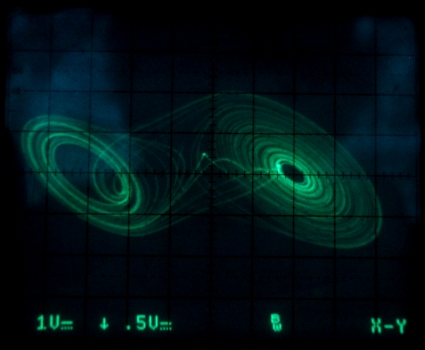
\includegraphics[scale = 0.5]{Images/real_chua.jpg}
        \caption{The output of an oscilloscope on a Chua's circuit.}
        \label{fig:my_label}
    \end{figure}

    With this in hand, we can simulate a variety of different initial conditions and constants to determine the expected results. An important factor to note is why exactly we would like to know that Chua's circuit follows chaotic behavior. 
    An issue that is prevalent within computer science as well as many computational methods is the deterministic behavior of computers. No number generated by the computer is truly random, and so we aim to change that. If we were able to implement a miniaturized version of Chua's circuit, it could be used as a random number generator, as the output voltages could be transformed and mapped as to generate a value between 0 and 1. However, the massive issue is that the system is deterministic - it is not truly random, as we were hoping for. However, if it were to be affected by background noise in some fashion, the output would be greatly changed, as we have shown within the prediction. Therefore, this chaotic system would be effectively random, and due to its simplicity, it would be a great candidate for a random number generator.
    
    There are some drawbacks to this simulation however. Within the physical implementation of the circuit, there is random noise, as discussed prior. In addition, the simulation does not account for the fact that any physical version of Chua's circuit would have non-ideal circuit components. However, these issues do not seem to have any significant impact, as the predictions and the actual results line up pretty close together. One thing to note though is that if the circuit were to get smaller and smaller, these issues would become more and more apparent and would have to be considered within the simulation. 
    
    An improvement that I would make now upon reflection would be an entire section towards how slight shifts in a single component could cause large changes in the end behavior. There are a large number of parameters, all of which affect the end results. Another possible addition would be to try combining multiple circuits, for which there has been research done on finding an analytical expression\footnote{https://doi.org/10.1142/S0218127403008697}. There are a number of uses for Chua's circuits\footnote{https://doi.org/10.1142/S0218126694000090}, and so studying its chaotic behavior may give us new insights into applications in a variety of fields.

\end{document}
